\documentclass{standalone}

\usepackage{tikz}
\usetikzlibrary{calc, arrows, chains, shapes.geometric}

\begin{document}
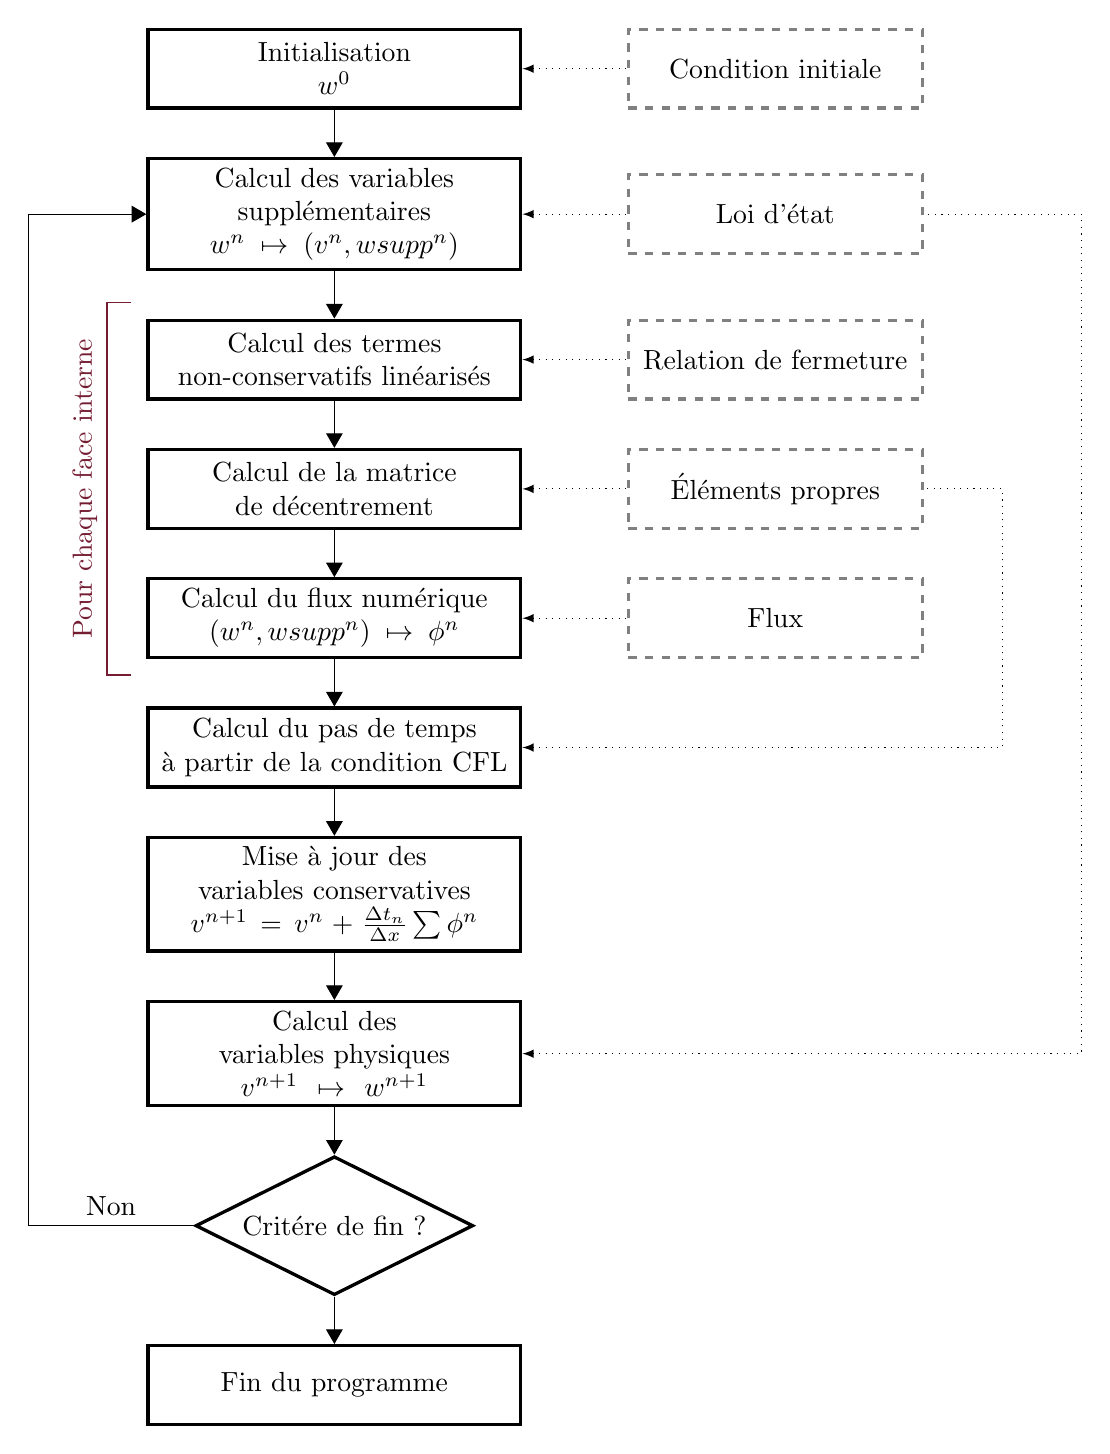
\begin{tikzpicture}
  [>=triangle 60,
    start chain=going below,
    node distance=6mm and 5cm,
    every join/.style={puis}]		

    \definecolor{bordeaux}{rgb}{0.454902, 0.113725, 0.196078} % Pantone 209

  \tikzset{
    base/.style={
      on chain, on grid,
      align=center,
      minimum height=1cm, 
    },
    process/.style={base,
      rectangle, 
      draw=black, very thick,
      text width=4.5cm, 
    }, 
    decision/.style={base,
      diamond,
      draw=black, very thick,
      aspect=2,
    }, 
    io/.style={base,
      rectangle, 
      draw=gray, very thick, dashed,
      text width=3.5cm, 
    }, 
    puis/.style={->, draw},
    avec/.style={latex-, draw, dotted},
  }

  \node[process] (init) {Initialisation\\$w^0$};
  \begin{scope}[start branch=ci]
    \node[io, right of=init, join=by avec] {Condition initiale};
  \end{scope}

  % \node[process, join] (AMR) {Si AMR :\\mise à jour du maillage};
  % \begin{scope}[start branch=AMR_criterion]
  % 	\node[io, right of=AMR, join=by avec] {Critère de raffinement};
  % \end{scope}

  \node[process, join] (wsupp) {Calcul des variables supplémentaires\\$w^n \mapsto (v^n, wsupp^n)$};
  \begin{scope}[start branch=EOS]
    \node[io, right of=wsupp, join=by avec] (EOS) {Loi d'état};
  \end{scope}
  
  % \node[process, join] (MUSCL) {Si MUSCL :\\extrapolation des variables};

  \node[process, join] (nc) {Calcul des termes\\non-conservatifs linéarisés};
  \begin{scope}[start branch=nc]
    \node[io, right of=nc, join=by avec] {Relation de fermeture};
  \end{scope}

  \node[process, join] (signe) {Calcul de la matrice de décentrement};
  \begin{scope}[start branch=eigen]
    \node[io, right of=signe, join=by avec] (eigen) {Éléments propres};
  \end{scope}
  
  \node[process, join] (flux) {Calcul du flux numérique\\$(w^n, wsupp^n) \mapsto \phi^n$};
  \begin{scope}[start branch=fluxes]
    \node[io, right of=flux, join=by avec] {Flux};
  \end{scope}

  \draw[bordeaux]
    % let \p1=(MUSCL.north west), \p2=(flux.south west) in
    let \p1=(nc.north west), \p2=(flux.south west) in
    (\x1-0.2cm, \y1+0.2cm) --  (\x1-0.5cm, \y1+0.2cm) --
    node[above, rotate=90] {Pour chaque face interne}
    (\x2-0.5cm, \y2-0.2cm) -- (\x2-0.2cm, \y2-0.2cm);

  \node[process, join] (cfl) {Calcul du pas de temps\\à partir de la condition CFL};
  \draw[avec]
    let \p1=(cfl.east), \p2=(eigen.east) in
    (\x1, \y1) --  (\x2+1cm, \y1) -- (\x2+1cm, \y2) -- (\x2, \y2);
  
  \node[process, join] (vnp1) {Mise à jour des\\variables conservatives\\$v^{n+1} = v^n + \frac{\Delta t_n}{\Delta x} \sum \phi^n$};

  \node[process, join] (invertEOS) {Calcul des\\variables physiques\\$v^{n+1} \mapsto w^{n+1} $};
  \draw[avec]
    let \p1=(invertEOS.east), \p2=(EOS.east) in
    (\x1, \y1) --  (\x2+2cm, \y1) -- (\x2+2cm, \y2) -- (\x2, \y2);

  % \node[process, join] (sauvegarde) {Enregistrement des données};

  \node[decision, join] (testfin) {Critére de fin ?};

  \draw[puis]
    % let \p1=(testfin.west), \p2=(AMR.west) in
    let \p1=(testfin.west), \p2=(wsupp.west) in
    (\x1, \y1) -- node[above] {Non} 
    (\x2-1.5cm, \y1) -- (\x2-1.5cm, \y2) -- (\x2, \y2);

  \node[process, join] (fin) {Fin du programme};
\end{tikzpicture}
\end{document}
